\documentclass[crop,tikz,border=2pt]{standalone}
\usetikzlibrary{patterns}
\newcommand{\tikzsetnextfilename}[1]{}
\definecolor{pBlue}{RGB}{86,139,190}
\definecolor{pOrange}{RGB}{211,153,80}
\definecolor{pPink}{RGB}{215,114,127}
\newcommand{\oldcells}[1]{%
  \foreach \x/\y in {#1}{%
    \ifnum\x>-1\relax
      \fill[pBlue!70!black] (\x,\y) rectangle ++(1,1);
      \draw[black!45,line width=.2pt] (\x,\y) rectangle ++(1,1);
    \fi
  }%
}
\newcommand{\itile}[1]{%
  \path[preaction={fill=pOrange!30},pattern=north east lines,
    pattern color=pOrange!90!black,draw=pOrange!80!black,line width=.5pt] #1;
}
\newcommand{\squarepattern}[1]{%
  \path[preaction={fill=pPink!25},pattern=crosshatch,
    pattern color=pPink!90!black,draw=pPink!80!black,line width=.5pt] #1;
}
\newcommand{\verticalI}{\itile{(0,0) rectangle (1,3)}}
\newcommand{\horizontalI}[2]{\itile{(0,#1) rectangle (3,#2)}}
\newcommand{\squaretile}[2]{\squarepattern{(0,#1) rectangle (2,#2)}}
% Each named picture becomes one SVG. Coordinates are measured from bottom left.
\begin{document}
\tikzsetnextfilename{transfer-matrix-triomino-profile-a}
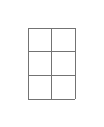
\begin{tikzpicture}[x=.3cm,y=.3cm]
\fill[white] (0,0) rectangle (2,3);
\oldcells{-1/-1}
\draw[step=1,black!55,line width=.25pt] (0,0) grid (2,3);
\end{tikzpicture}
\tikzsetnextfilename{transfer-matrix-triomino-profile-b}
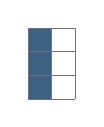
\begin{tikzpicture}[x=.3cm,y=.3cm]
\fill[white] (0,0) rectangle (2,3);
\oldcells{0/0,0/1,0/2}
\draw[step=1,black!55,line width=.25pt] (0,0) grid (2,3);
\end{tikzpicture}
\tikzsetnextfilename{transfer-matrix-triomino-profile-c}
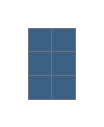
\begin{tikzpicture}[x=.3cm,y=.3cm]
\fill[white] (0,0) rectangle (2,3);
\oldcells{0/0,0/1,0/2,1/0,1/1,1/2}
\draw[step=1,black!55,line width=.25pt] (0,0) grid (2,3);
\end{tikzpicture}
\tikzsetnextfilename{transfer-matrix-triomino-profile-d}
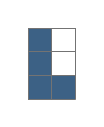
\begin{tikzpicture}[x=.3cm,y=.3cm]
\fill[white] (0,0) rectangle (2,3);
\oldcells{0/0,0/1,0/2,1/0}
\draw[step=1,black!55,line width=.25pt] (0,0) grid (2,3);
\end{tikzpicture}
\tikzsetnextfilename{transfer-matrix-triomino-profile-e}
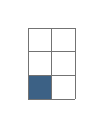
\begin{tikzpicture}[x=.3cm,y=.3cm]
\fill[white] (0,0) rectangle (2,3);
\oldcells{0/0}
\draw[step=1,black!55,line width=.25pt] (0,0) grid (2,3);
\end{tikzpicture}
\tikzsetnextfilename{transfer-matrix-triomino-profile-f}
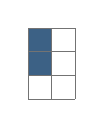
\begin{tikzpicture}[x=.3cm,y=.3cm]
\fill[white] (0,0) rectangle (2,3);
\oldcells{0/1,0/2}
\draw[step=1,black!55,line width=.25pt] (0,0) grid (2,3);
\end{tikzpicture}
\tikzsetnextfilename{transfer-matrix-triomino-profile-g}
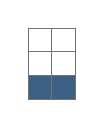
\begin{tikzpicture}[x=.3cm,y=.3cm]
\fill[white] (0,0) rectangle (2,3);
\oldcells{0/0,1/0}
\draw[step=1,black!55,line width=.25pt] (0,0) grid (2,3);
\end{tikzpicture}
\tikzsetnextfilename{transfer-matrix-triomino-profile-h}
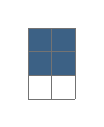
\begin{tikzpicture}[x=.3cm,y=.3cm]
\fill[white] (0,0) rectangle (2,3);
\oldcells{0/1,0/2,1/1,1/2}
\draw[step=1,black!55,line width=.25pt] (0,0) grid (2,3);
\end{tikzpicture}
\tikzsetnextfilename{transfer-matrix-triomino-profile-i}
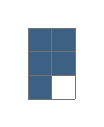
\begin{tikzpicture}[x=.3cm,y=.3cm]
\fill[white] (0,0) rectangle (2,3);
\oldcells{0/0,0/1,0/2,1/1,1/2}
\draw[step=1,black!55,line width=.25pt] (0,0) grid (2,3);
\end{tikzpicture}
\tikzsetnextfilename{transfer-matrix-triomino-transition-aa}
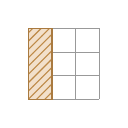
\begin{tikzpicture}[x=.3cm,y=.3cm]
\fill[white] (0,0) rectangle (3,3);
\draw[step=1,black!40,line width=.2pt] (0,0) grid (3,3);
\oldcells{-1/-1}
\verticalI
\end{tikzpicture}
\tikzsetnextfilename{transfer-matrix-triomino-transition-ac}
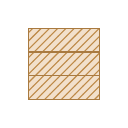
\begin{tikzpicture}[x=.3cm,y=.3cm]
\fill[white] (0,0) rectangle (3,3);
\draw[step=1,black!40,line width=.2pt] (0,0) grid (3,3);
\oldcells{-1/-1}
\horizontalI{0}{1}\horizontalI{1}{2}\horizontalI{2}{3}
\end{tikzpicture}
\tikzsetnextfilename{transfer-matrix-triomino-transition-ad}
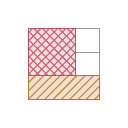
\begin{tikzpicture}[x=.3cm,y=.3cm]
\fill[white] (0,0) rectangle (3,3);
\draw[step=1,black!40,line width=.2pt] (0,0) grid (3,3);
\oldcells{-1/-1}
\horizontalI{0}{1}\squaretile{1}{3}
\end{tikzpicture}
\tikzsetnextfilename{transfer-matrix-triomino-transition-ba}
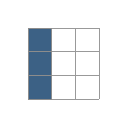
\begin{tikzpicture}[x=.3cm,y=.3cm]
\fill[white] (0,0) rectangle (3,3);
\draw[step=1,black!40,line width=.2pt] (0,0) grid (3,3);
\oldcells{0/0,0/1,0/2}

\end{tikzpicture}
\tikzsetnextfilename{transfer-matrix-triomino-transition-cb}
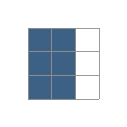
\begin{tikzpicture}[x=.3cm,y=.3cm]
\fill[white] (0,0) rectangle (3,3);
\draw[step=1,black!40,line width=.2pt] (0,0) grid (3,3);
\oldcells{0/0,0/1,0/2,1/0,1/1,1/2}

\end{tikzpicture}
\tikzsetnextfilename{transfer-matrix-triomino-transition-de}
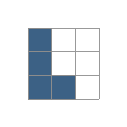
\begin{tikzpicture}[x=.3cm,y=.3cm]
\fill[white] (0,0) rectangle (3,3);
\draw[step=1,black!40,line width=.2pt] (0,0) grid (3,3);
\oldcells{0/0,0/1,0/2,1/0}

\end{tikzpicture}
\tikzsetnextfilename{transfer-matrix-triomino-transition-ef}
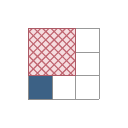
\begin{tikzpicture}[x=.3cm,y=.3cm]
\fill[white] (0,0) rectangle (3,3);
\draw[step=1,black!40,line width=.2pt] (0,0) grid (3,3);
\oldcells{0/0}
\squaretile{1}{3}
\end{tikzpicture}
\tikzsetnextfilename{transfer-matrix-triomino-transition-eh}
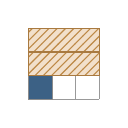
\begin{tikzpicture}[x=.3cm,y=.3cm]
\fill[white] (0,0) rectangle (3,3);
\draw[step=1,black!40,line width=.2pt] (0,0) grid (3,3);
\oldcells{0/0}
\horizontalI{1}{2}\horizontalI{2}{3}
\end{tikzpicture}
\tikzsetnextfilename{transfer-matrix-triomino-transition-fg}
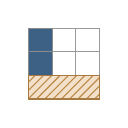
\begin{tikzpicture}[x=.3cm,y=.3cm]
\fill[white] (0,0) rectangle (3,3);
\draw[step=1,black!40,line width=.2pt] (0,0) grid (3,3);
\oldcells{0/1,0/2}
\horizontalI{0}{1}
\end{tikzpicture}
\tikzsetnextfilename{transfer-matrix-triomino-transition-gb}
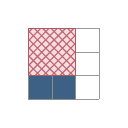
\begin{tikzpicture}[x=.3cm,y=.3cm]
\fill[white] (0,0) rectangle (3,3);
\draw[step=1,black!40,line width=.2pt] (0,0) grid (3,3);
\oldcells{0/0,1/0}
\squaretile{1}{3}
\end{tikzpicture}
\tikzsetnextfilename{transfer-matrix-triomino-transition-gi}
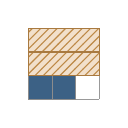
\begin{tikzpicture}[x=.3cm,y=.3cm]
\fill[white] (0,0) rectangle (3,3);
\draw[step=1,black!40,line width=.2pt] (0,0) grid (3,3);
\oldcells{0/0,1/0}
\horizontalI{1}{2}\horizontalI{2}{3}
\end{tikzpicture}
\tikzsetnextfilename{transfer-matrix-triomino-transition-hd}
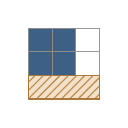
\begin{tikzpicture}[x=.3cm,y=.3cm]
\fill[white] (0,0) rectangle (3,3);
\draw[step=1,black!40,line width=.2pt] (0,0) grid (3,3);
\oldcells{0/1,0/2,1/1,1/2}
\horizontalI{0}{1}
\end{tikzpicture}
\tikzsetnextfilename{transfer-matrix-triomino-transition-if}
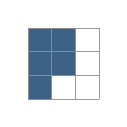
\begin{tikzpicture}[x=.3cm,y=.3cm]
\fill[white] (0,0) rectangle (3,3);
\draw[step=1,black!40,line width=.2pt] (0,0) grid (3,3);
\oldcells{0/0,0/1,0/2,1/1,1/2}

\end{tikzpicture}
\end{document}
